\chapter{इलेक्ट्रॉनिक स्पेक्ट्रमिकी और प्रकाशभौतिकी}\label{ch:b3:electronic-spectroscopy}

किसी अँधेरे बार के पराबैंगनी लैंप के नीचे टॉनिक जल का गिलास फीकी, प्रेत-सी
नीली आभा से चमकता है। उसमें घुली क्विनीन पराबैंगनी प्रकाश अवशोषित करती है, जिसे
आँख नहीं देख सकती, और उसका कुछ भाग कुछ नैनोसेकंड बाद दृश्य नीले प्रकाश के रूप में
लौटा देती है। अवशोषण, उत्तेजित अवस्था में एक छोटा जीवन, लंबे तरंगदैर्घ्य पर
उत्सर्जन, और वह ऊर्जा जो प्रकाश के रूप में नहीं लौटती: उत्तेजित अणु की नियति
दर स्थिरांकों वाले प्रक्रमों के बीच एक प्रतिस्पर्धा है, और उसका स्पेक्ट्रम अणु के
कंपनों और \cref{ch:b3:group-theory-applied} के सममिति नियमों से आकार लेता है। यह अध्याय
इलेक्ट्रॉनिक संक्रमणों का और उनके बाद होने वाली घटनाओं का अध्ययन करता है, जिस विषय को
प्रकाशभौतिकी कहते हैं; \cref{ch:b3:photochemistry} वे स्थितियाँ जोड़ता है जिनमें उत्तेजित
अणु अभिक्रिया करता है।

\begin{recall}
प्रथम वर्ष के खंड ने बियर--लैंबर्ट नियम, $A =
\varepsilon\ell c$, से अवशोषकता मापी, मोलर अवशोषण गुणांक, वर्णमूलक और
संयुग्मित तंत्र परिभाषित किए, और रंग को अवशोषण अधिकतम से जोड़ा। द्वितीय वर्ष के
खंड ने अग्रांत कक्षकों HOMO और LUMO को नाम दिया। \Cref{ch:b3:many-electron-atoms}
ने एकल और \omterm{def:b3:many-electron-atoms:singlet-triplet}{त्रिक अवस्थाएँ} परिभाषित कीं; \cref{ch:b3:group-theory-applied} ने
लुप्त होने वाले समाकलों का प्रमेय; \cref{ch:b3:rovibrational-spectroscopy} ने किसी
आबंध के कंपनिक स्तर।
\end{recall}

\begin{omfigure}
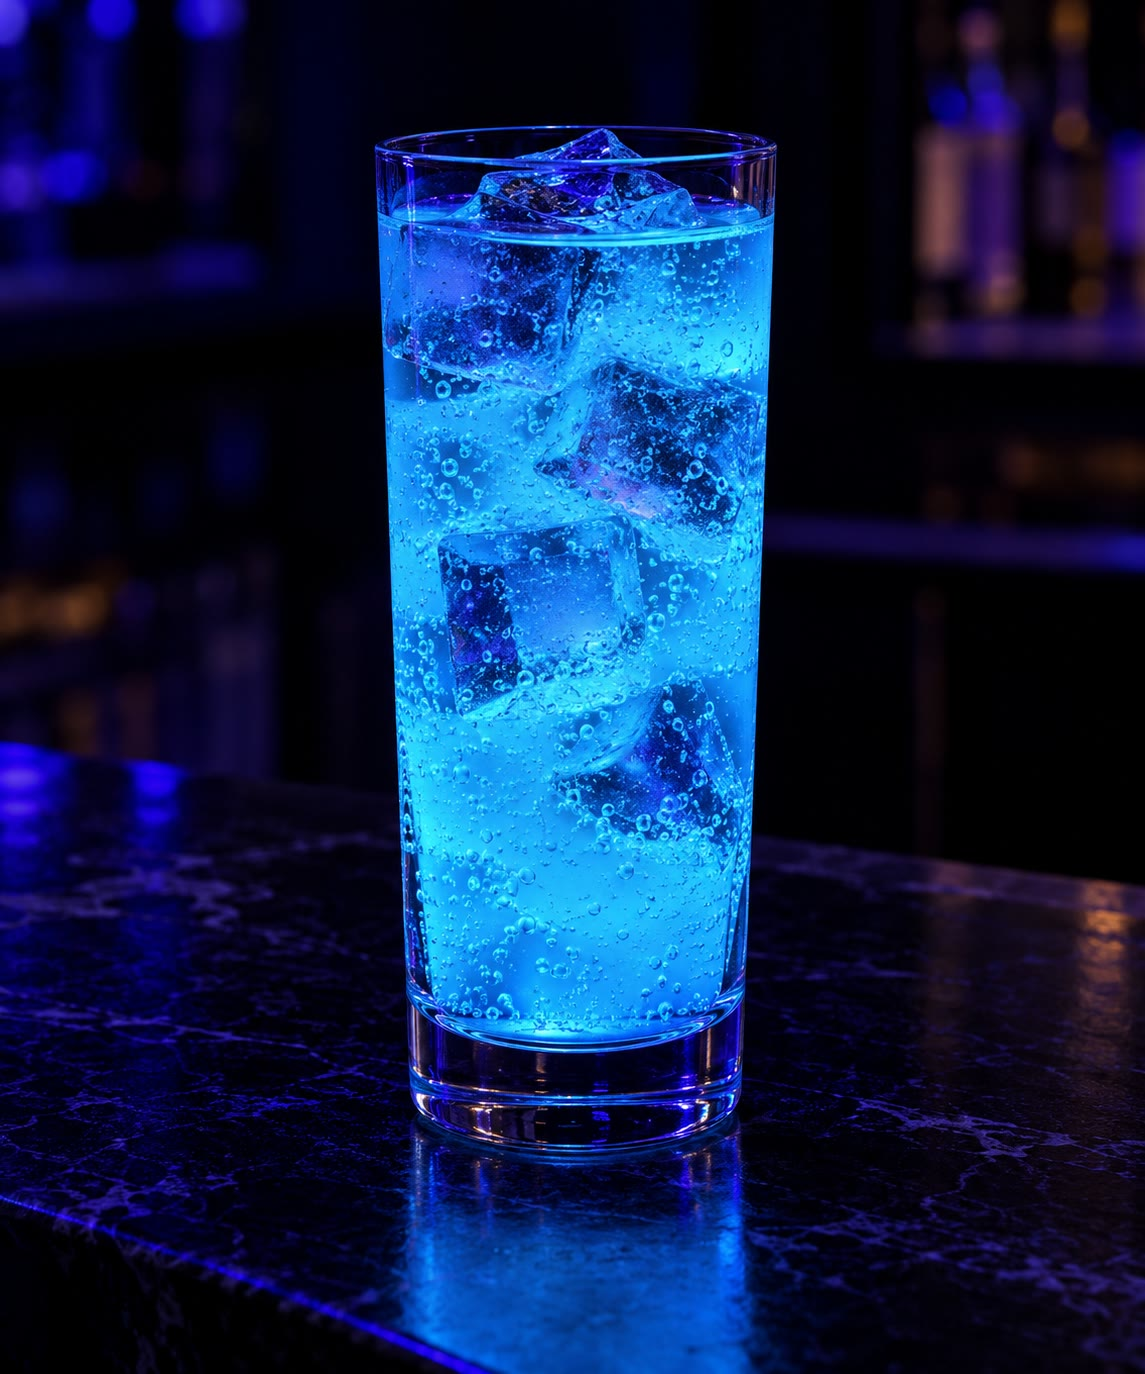
\includegraphics[height=4.6cm]{images/book4/ai/b3-07-tonic.jpg}\hspace{1em}%
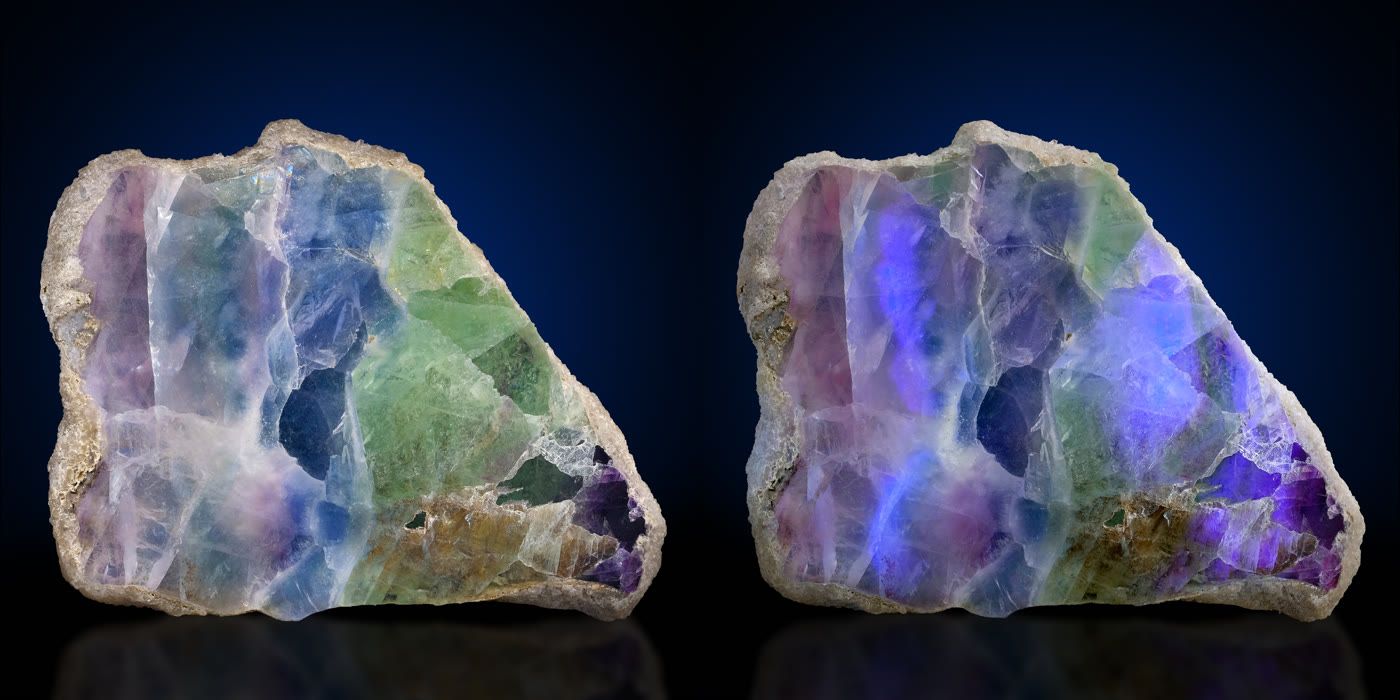
\includegraphics[height=4.6cm]{images/book4/fluorite-uv.jpg}

{\small बाएँ: पराबैंगनी लैंप के नीचे नीला चमकता टॉनिक जल। दाएँ:
दिन के प्रकाश में फ़्लोराइट, और पराबैंगनी प्रकाश में प्रतिदीप्त होता फ़्लोराइट; इसी
खनिज ने \omterm{def:b3:electronic-spectroscopy:luminescence}{प्रतिदीप्ति} को उसका नाम दिया। (छायाचित्र: माशा मिल्शिना, CC BY 4.0।)}
\end{omfigure}

\section{इलेक्ट्रॉनिक संक्रमण और उनके वरण नियम}

\begin{definition}[संक्रमण द्विध्रुव आघूर्ण, दोलक सामर्थ्य]\label{def:b3:electronic-spectroscopy:transition-dipole}
अवस्थाओं $\Psi_i$ और $\Psi_f$ के बीच \emph{संक्रमण द्विध्रुव आघूर्ण}\index{संक्रमण द्विध्रुव आघूर्ण}
$\boldsymbol\mu_{fi} = \langle\Psi_f|\hat{\boldsymbol\mu}|\Psi_i
\rangle$ है, जहाँ $\hat{\boldsymbol\mu} = -e\sum_k\mathbf r_k$ (साथ में नाभिकीय
आवेश, जो लांबिक अवस्थाओं के बीच निरस्त हो जाते हैं)। \emph{दोलक
सामर्थ्य}\index{दोलक सामर्थ्य} $f$ किसी बैंड की तीव्रता का विमाहीन माप है,
सबसे प्रबल संक्रमणों के लिए लगभग 1।
\end{definition}

\begin{proposition}[तीव्रता और दोलक सामर्थ्य]\label{prop:b3:electronic-spectroscopy:intensity}
किसी बैंड का समाकलित अवशोषण $|\boldsymbol\mu_{fi}|^2$ के समानुपाती है,
और व्यवहार में
\[
f \approx 4.32\times10^{-9}\int\varepsilon(\tilde\nu)\,\dd\tilde\nu,
\]
जहाँ $\varepsilon$, \unit{L.mol^{-1}.cm^{-1}} में और $\tilde\nu$, \unit{cm^{-1}} में है।
\end{proposition}
\admitted

समानुपातिता काल-आश्रित विक्षोभ सिद्धांत से आती है और
संख्यात्मक गुणक चिरसम्मत दोलक से; दोनों अधिक उन्नत पाठ्यक्रमों में दिए जाते हैं।
यहाँ महत्वपूर्ण यह है कि $f$ तभी बड़ा होता है जब
$\boldsymbol\mu_{fi}$ बड़ा हो, और सममिति उसे शून्य होने पर विवश कर सकती है।

\begin{theorem}[चक्रण वरण नियम]\label{thm:b3:electronic-spectroscopy:spin-rule}
भिन्न कुल चक्रण वाली अवस्थाओं के बीच विद्युत-द्विध्रुव संक्रमण
वर्जित है: $\Delta S = 0$।
\end{theorem}

\begin{proof}
हर अवस्था एक आकाशी और एक चक्रण फलन का गुणनफल है, $\Psi = \phi\,\chi$।
द्विध्रुव \omterm{def:b3:quantum-model-systems:operator}{संकारक} केवल स्थितियों पर क्रिया करता है, अतः $\langle\phi_f\chi_f|\hat{\boldsymbol\mu}|
\phi_i\chi_i\rangle = \langle\phi_f|\hat{\boldsymbol\mu}|\phi_i\rangle\langle\chi_f|\chi_i\rangle$।
भिन्न $S$ वाले चक्रण फलन $\hat S^2$ के भिन्न \omterm{def:b3:quantum-model-systems:operator}{अभिलक्षणिक मानों} वाले \omterm{def:b3:quantum-model-systems:operator}{अभिलक्षणिक फलन} हैं,
अतः लांबिक (\cref{thm:b3:quantum-model-systems:hermitian-real}):
दूसरा गुणक लुप्त हो जाता है।
\end{proof}

\begin{theorem}[लापोर्ट नियम]\label{thm:b3:electronic-spectroscopy:laporte}
\omterm{def:b3:point-groups:inversion}{प्रतिलोमन केंद्र} वाले अणु में विद्युत-द्विध्रुव संक्रमण को
समता बदलनी ही चाहिए: $g \leftrightarrow u$ अनुमत है, $g \leftrightarrow g$ और $u
\leftrightarrow u$ वर्जित हैं। यही \emph{लापोर्ट नियम}\index{लापोर्ट नियम} है।
\end{theorem}

\begin{proof}
$\hat{\boldsymbol\mu}$ के घटक प्रतिलोमन के अंतर्गत चिह्न बदलते हैं: वे $u$ हैं।
गुणनफल $\Gamma_f\otimes\Gamma_\mu\otimes\Gamma_i$ केवल तभी $g$ है जब $\Gamma_f$ और $\Gamma_i$
की समताएँ विपरीत हों; अन्यथा वह $u$ है और उसमें \omterm{def:b3:group-theory-applied:reducible}{पूर्णतः
सममित निरूपण} नहीं हो सकता (\cref{thm:b3:group-theory-applied:vanishing-integral})।
\end{proof}

दोनों नियम आदर्शीकृत अवस्थाओं के लिए कठोर हैं; वास्तविक अणु उन्हें शिथिल कर देते हैं
--- \omterm{def:b3:many-electron-atoms:spin-orbit}{चक्रण--कक्षक युग्मन} एकल और त्रिक स्वरूप को मिश्रित करता है, कंपन
क्षण भर के लिए सममिति केंद्र को हटा देते हैं --- और ``वर्जित''
संक्रमण दुर्बल रूप में प्रकट होते हैं। अष्टफलकीय संकुलों के $d$--$d$ बैंड, जो लापोर्ट
वर्जित और दुर्बल हैं, अपना रंग इसी शिथिलन के कारण पाते हैं
(\cref{ch:b3:complex-spectra-magnetism})।

\begin{definition}[आवेश-स्थानांतरण संक्रमण]\label{def:b3:electronic-spectroscopy:charge-transfer}
\emph{आवेश-स्थानांतरण संक्रमण}\index{आवेश-स्थानांतरण संक्रमण} किसी इलेक्ट्रॉन को
ऐसे कक्षक से, जो मुख्यतः किसी तंत्र के एक भाग (दाता) पर स्थित है, ऐसे कक्षक में ले जाता है
जो मुख्यतः दूसरे भाग (ग्राही) पर स्थित है; उसका संक्रमण द्विध्रुव
बड़ा, उसका बैंड तीव्र और चौड़ा, और उसकी ऊर्जा विलायक की ध्रुवता के प्रति
संवेदनशील होती है।
\end{definition}

\begin{method}[अवशोषण बैंड का निर्धारण]\label{met:b3:electronic-spectroscopy:assign-band}
\begin{enumerate}
  \item $\varepsilon_{\max}$ लगभग \qty{e4}{L.mol^{-1}.cm^{-1}} से ऊपर: एक अनुमत
        संक्रमण (संयुग्मित तंत्र का $\pi\to\pi^*$, या आवेश स्थानांतरण)।
  \item $\varepsilon_{\max}$ 10 से कुछ सौ तक: एक वर्जित संक्रमण ($n\to\pi^*$,
        सममिति-वर्जित; $d$--$d$, लापोर्ट-वर्जित)।
  \item $\varepsilon_{\max}$ 1 से कम: चक्रण-वर्जित।
  \item $n\to\pi^*$ बैंड प्रोटिक विलायकों में छोटे तरंगदैर्घ्यों की ओर खिसकता है
        (एकाकी युग्म हाइड्रोजन आबंधों से स्थायीकृत होता है), $\pi\to\pi^*$ बैंड
        प्रायः लंबे तरंगदैर्घ्यों की ओर।
\end{enumerate}
\end{method}

\section{फ़्रैंक--कॉन्डन सिद्धांत}

\begin{theorem}[फ़्रैंक--कॉन्डन सिद्धांत]\label{thm:b3:electronic-spectroscopy:franck-condon}
\omterm{def:b3:computational-chemistry:born-oppenheimer}{बॉर्न--ओपेनहाइमर सन्निकटन} के भीतर, और यदि संक्रमण द्विध्रुव
नाभिकीय स्थितियों पर कम निर्भर करता हो, तो \omterm{def:b3:electronic-spectroscopy:vibronic}{कंपन-इलेक्ट्रॉनिक
संक्रमण} की तीव्रता, निचली इलेक्ट्रॉनिक अवस्था के कंपनिक स्तर $v''$ से ऊपरी अवस्था के स्तर
$v'$ तक, $|\langle\chi_{v'}|\chi_{v''}\rangle|^2$ के समानुपाती है, जो
दोनों कंपनिक तरंग फलनों के अतिव्यापन का वर्ग है: यही
\emph{फ़्रैंक--कॉन्डन सिद्धांत}\index{फ़्रैंक--कॉन्डन सिद्धांत} है। इलेक्ट्रॉनिक
संक्रमण ऊर्ध्वाधर होते हैं: इलेक्ट्रॉनों की छलाँग के दौरान नाभिक नहीं हिलते।
\end{theorem}

\begin{proof}
$\Psi = \psi_{\mathrm{el}}(\mathbf r;R)\chi_v(R)$ के साथ संक्रमण आघूर्ण
$\int\chi_{v'}^*\big[\int\psi'^*_{\mathrm{el}}\hat\mu\psi''_{\mathrm{el}}\dd\mathbf r\big]
\chi_{v''}\,\dd R$ है। कोष्ठक इलेक्ट्रॉनिक संक्रमण आघूर्ण
$\mu_{\mathrm{el}}(R)$ है; अचर मानने पर (कॉन्डन सन्निकटन), वह
समाकल से बाहर आ जाता है, और $\mu_{\mathrm{el}}\langle\chi_{v'}|\chi_{v''}\rangle$ बचता है।
\end{proof}

\begin{definition}[कंपन-इलेक्ट्रॉनिक संक्रमण, श्रेणी, फ़्रैंक--कॉन्डन गुणक]\label{def:b3:electronic-spectroscopy:vibronic}
\emph{कंपन-इलेक्ट्रॉनिक संक्रमण}\index{कंपन-इलेक्ट्रॉनिक संक्रमण} इलेक्ट्रॉनिक
और कंपनिक अवस्थाओं को साथ-साथ बदलता है; रेखाएँ $v' \leftarrow 0$, जहाँ $v' = 0, 1, 2,
\dots$, एक \emph{कंपन-इलेक्ट्रॉनिक श्रेणी}\index{कंपन-इलेक्ट्रॉनिक श्रेणी} बनाती हैं; किसी
कंपन-इलेक्ट्रॉनिक रेखा का \emph{फ़्रैंक--कॉन्डन गुणक}\index{फ़्रैंक--कॉन्डन गुणक}
$|\langle\chi_{v'}|\chi_{v''}\rangle|^2$ है।
\end{definition}

\begin{proposition}[विस्थापित दोलित्र]\label{prop:b3:electronic-spectroscopy:displaced}
यदि दोनों अवस्थाएँ समान आवृत्ति के साथ आवर्ती हैं और ऊपरी निम्निष्ठ
$\Delta$ ($\sqrt{\hbar/m\omega}$ की इकाइयों में) से विस्थापित है, तो $v'' = 0$ से \omterm{def:b3:electronic-spectroscopy:vibronic}{फ़्रैंक--कॉन्डन
गुणक} एक प्वासों वितरण बनाते हैं,
$|\langle v'|0\rangle|^2 = \eu^{-S}S^{v'}/v'!$, जहाँ $S = \Delta^2/2$; सबसे प्रबल रेखा
$v' = S$ के निकट होती है।
\end{proposition}
\admitted

सामान्य उपपत्ति \cref{ch:b3:quantum-model-systems} के \omterm{def:b3:quantum-model-systems:ladder}{सीढ़ी संकारकों} का उपयोग
करती है; इस अध्याय के चित्र-आँकड़े सूत्र की जाँच प्रत्यक्ष समाकलन से करते हैं।
छोटा विस्थापन एक प्रबल 0--0 रेखा देता है; बड़ा विस्थापन एक लंबी श्रेणी, जिसका
सबसे प्रबल सदस्य 0--0 रेखा से दूर होता है।

\begin{omfigure}
\begin{tikzpicture}
\begin{axis}[name=pc, width=0.46\linewidth, height=6cm, xmin=-4, xmax=5, ymin=0,
  ymax=14, axis lines=left, xtick=\empty, ytick=\empty, xlabel={नाभिकीय निर्देशांक},
  ylabel={ऊर्जा}, label style={font=\small}]
\addplot[black, thick] table[x=y, y=ground] {figdata/out/bachelor-3-franck-condon-curves.dat};
\addplot[omDef, thick] table[x=y, y=excited] {figdata/out/bachelor-3-franck-condon-curves.dat};
\draw[omabs] (axis cs:0,0.5) -- (axis cs:0,10.6);
\draw[omvib] (axis cs:-1,0.5) -- (axis cs:1,0.5);
\draw[omvib] (axis cs:0.732,9.5) -- (axis cs:2.732,9.5);
\draw[omvib] (axis cs:-0.000,10.5) -- (axis cs:3.464,10.5);
\draw[omvib] (axis cs:-0.504,11.5) -- (axis cs:3.968,11.5);
\draw[omvib] (axis cs:-0.914,12.5) -- (axis cs:4.378,12.5);
\node[font=\small, anchor=west] at (axis cs:-3.9,13.0) {उत्तेजित};
\node[font=\small, anchor=west] at (axis cs:3.0,1.5) {मूल};
\node[font=\scriptsize, anchor=east] at (axis cs:-0.05,5.5) {ऊर्ध्वाधर};
\end{axis}
\begin{axis}[at={(pc.east)}, anchor=west, xshift=1.3cm, width=0.46\linewidth,
  height=6cm, xmin=-0.5, xmax=12.5, ymin=0, ymax=0.8, axis lines=left, ycomb,
  xlabel={$v'$}, ylabel={फ़्रैंक--कॉन्डन गुणक}, label style={font=\small},
  tick label style={font=\small}]
\addplot[black, very thick] table[x=v, y=s03] {figdata/out/bachelor-3-franck-condon-sticks.dat};
\addplot[omDef, very thick, xshift=2pt] table[x=v, y=s15] {figdata/out/bachelor-3-franck-condon-sticks.dat};
\addplot[omThm, very thick, xshift=4pt] table[x=v, y=s5] {figdata/out/bachelor-3-franck-condon-sticks.dat};
\end{axis}
\end{tikzpicture}

{\small बाएँ: मूल अवस्था के निम्नतम स्तर से एक ऊर्ध्वाधर संक्रमण वहाँ
पहुँचता है जहाँ उत्तेजित वक्र, जो लंबी आबंध लंबाई की ओर विस्थापित है, अपने निम्निष्ठ से बहुत
ऊपर है ($S = 1.5$ के लिए खींचा गया)। दाएँ: श्रेणी के \omterm{def:b3:electronic-spectroscopy:vibronic}{फ़्रैंक--कॉन्डन गुणक},
$S = 0.3$ (काला), 1.5 (नीला) और 5 (लाल) के लिए; हर समुच्चय का योग
1 है।}
\end{omfigure}

\begin{example}[आयोडीन]\label{ex:b3:electronic-spectroscopy:iodine}
% ledger: diat:I2.re, diat:I2B.re, diat:I2B.we, imass:I127
आयोडीन वाष्प बैंगनी है क्योंकि उसका B$\leftarrow$X बैंड पीला-हरा प्रकाश अवशोषित करता है।
आबंध मूल अवस्था में \qty{266.6}{pm} से बढ़कर
B अवस्था में \qty{302.5}{pm} हो जाता है। B-अवस्था की आवृत्ति
(\qty{125.7}{cm^{-1}}) के साथ विस्थापित-दोलित्र मॉडल में, $\Delta R = \qty{35.8}{pm}$ से $S \approx 15$ मिलता है: अवशोषण
एक लंबी श्रेणी है, जिसकी सबसे प्रबल रेखाएँ B अवस्था के ऊँचे कंपनिक स्तरों पर
समाप्त होती हैं, और जिसका विस्तार वियोजन सांतत्य में चला जाता है।
\end{example}

\section{उत्तेजित अवस्था की नियतियाँ: याब्लोन्स्की आरेख}

\begin{definition}[याब्लोन्स्की आरेख]\label{def:b3:electronic-spectroscopy:jablonski}
\emph{याब्लोन्स्की आरेख}\index{याब्लोन्स्की आरेख} किसी अणु की इलेक्ट्रॉनिक अवस्थाएँ
(एकल $S_0, S_1, S_2, \dots$ एक स्तंभ में, त्रिक $T_1, T_2,
\dots$ दूसरे में), उनके कंपनिक स्तर, और उन्हें जोड़ने वाले प्रक्रम दिखाता है:
विकिरणी प्रक्रम सीधे तीरों से, अविकिरणी प्रक्रम लहरदार तीरों से।
\end{definition}

\begin{definition}[अविकिरणी प्रक्रम]\label{def:b3:electronic-spectroscopy:radiationless}
\emph{कंपनिक विश्रांति}\index{कंपनिक विश्रांति} उत्तेजित अणु को
संघट्टों द्वारा, पिकोसेकंडों में, उसकी इलेक्ट्रॉनिक अवस्था के निम्नतम कंपनिक स्तर पर ले आती है।
\emph{आंतरिक रूपांतरण}\index{आंतरिक रूपांतरण}
समान बहुकता वाली अवस्थाओं के बीच एक अविकिरणी संक्रमण है
($S_2 \to S_1$, $S_1 \to S_0$); \emph{अंतरतंत्र
संक्रमण}\index{अंतरतंत्र संक्रमण} भिन्न बहुकता वाली अवस्थाओं के बीच
($S_1 \to T_1$, $T_1 \to S_0$)।
\end{definition}

\begin{definition}[संदीप्ति, प्रतिदीप्ति, स्फुरदीप्ति, स्टोक्स विस्थापन]\label{def:b3:electronic-spectroscopy:luminescence}
\emph{संदीप्ति}\index{संदीप्ति} उत्तेजित अणु द्वारा प्रकाश का उत्सर्जन है।
\emph{प्रतिदीप्ति}\index{प्रतिदीप्ति} चक्रण-अनुमत उत्सर्जन है,
प्रायः $S_1 \to S_0$, तीव्र (नैनोसेकंड); \emph{स्फुरदीप्ति}\index{स्फुरदीप्ति}
चक्रण-वर्जित उत्सर्जन है, प्रायः $T_1 \to S_0$, मंद (मिलीसेकंडों से
सेकंडों तक)। \emph{स्टोक्स विस्थापन}\index{स्टोक्स विस्थापन} अवशोषण और उत्सर्जन
अधिकतमों के बीच का अंतर है, ऊर्जा में।
\end{definition}

\begin{omfigure}
\begin{tikzpicture}[font=\small, >=Stealth]
  \foreach \y/\l in {0/{$S_0$}, 3.4/{$S_1$}, 5.6/{$S_2$}}{
    \draw[omstate] (0,\y) -- (3.6,\y); \node[anchor=east] at (-0.1,\y) {\l};
    \foreach \d in {0.25,0.5,0.75}{\draw[omvib] (0,\y+\d) -- (3.6,\y+\d);}}
  \draw[omstate] (5.0,2.5) -- (7.6,2.5); \node[anchor=west] at (7.7,2.5) {$T_1$};
  \foreach \d in {0.25,0.5,0.75}{\draw[omvib] (5.0,2.5+\d) -- (7.6,2.5+\d);}
  \draw[omabs] (0.3,0) -- (0.3,4.15) node[pos=0.35, left, font=\scriptsize, align=right] {अवशोषण};
  \draw[omabs] (0.7,0) -- (0.7,5.85);
  \draw[omnonrad] (1.05,5.85) -- (1.05,5.6);
  \draw[omnonrad] (1.05,5.6) -- (1.05,3.4) node[pos=0.5, right, font=\scriptsize] {IC};
  \draw[omnonrad] (0.45,4.15) -- (0.45,3.42);
  \draw[omfluo] (1.7,3.4) -- (1.7,0.5) node[pos=0.5, right, font=\scriptsize, align=left] {प्रति-\\दीप्ति};
  \draw[omnonrad] (3.2,3.4) -- (3.2,0.02) node[pos=0.5, right, font=\scriptsize] {IC};
  \draw[omisc] (3.6,3.4) -- (5.0,3.1) node[pos=0.5, above, font=\scriptsize] {ISC};
  \draw[omnonrad] (5.3,3.1) -- (5.3,2.52);
  \draw[omphos] (6.0,2.5) -- (6.0,0.5) node[pos=0.5, right, font=\scriptsize, align=left] {स्फुर-\\दीप्ति};
  \draw[omisc] (5.6,2.5) -- (3.7,0.02) node[pos=0.45, above left, font=\scriptsize, inner sep=1pt] {ISC};
  \draw[omvib, dashed] (3.6,0.5) -- (6.0,0.5);
  \draw[omvib, dashed] (3.6,0.0) -- (7.6,0.0);
\end{tikzpicture}

{\small एक \omterm{def:b3:electronic-spectroscopy:jablonski}{याब्लोन्स्की आरेख}। सीधे तीर: अवशोषण (नीला), \omterm{def:b3:electronic-spectroscopy:luminescence}{प्रतिदीप्ति}
(लाल), \omterm{def:b3:electronic-spectroscopy:luminescence}{स्फुरदीप्ति} (नारंगी); लहरदार तीर: \omterm{def:b3:electronic-spectroscopy:radiationless}{कंपनिक विश्रांति} और
\omterm{def:b3:electronic-spectroscopy:radiationless}{आंतरिक रूपांतरण} (IC); खंडित लहरदार तीर: \omterm{def:b3:electronic-spectroscopy:radiationless}{अंतरतंत्र संक्रमण} (ISC)।
उत्सर्जन $S_1$ या $T_1$ के निम्नतम कंपनिक स्तर से आरंभ होता है और
$S_0$ के किसी भी स्तर पर समाप्त हो सकता है।}
\end{omfigure}

\begin{proposition}[काशा का नियम]\label{prop:b3:electronic-spectroscopy:kasha}
\omterm{def:b3:electronic-spectroscopy:luminescence}{संदीप्ति}, बहुत कम अपवादों के साथ, दी हुई बहुकता की निम्नतम उत्तेजित अवस्था
($S_1$ या $T_1$) से होती है, चाहे पहले कोई भी अवस्था उत्तेजित हुई हो:
यही \emph{काशा का नियम}\index{काशा का नियम} है।
\end{proposition}
\begin{proof}[स्थिति]
प्रायोगिक रूप से स्थापित; कारण यह है कि ऊपरी उत्तेजित अवस्थाओं के बीच, जो
पास-पास हैं, \omterm{def:b3:electronic-spectroscopy:radiationless}{आंतरिक रूपांतरण} उत्सर्जन से कहीं तीव्र है,
जबकि अंतराल $S_1$--$S_0$ बड़ा है।
\end{proof}

\begin{proposition}[दर्पण-प्रतिबिंब]\label{prop:b3:electronic-spectroscopy:mirror}
यदि उत्तेजित और मूल अवस्थाओं की कंपनिक संरचना समान हो, तो
\omterm{def:b3:electronic-spectroscopy:luminescence}{प्रतिदीप्ति} बैंड पहले अवशोषण बैंड का उनकी उभयनिष्ठ 0--0 रेखा के सापेक्ष
दर्पण-प्रतिबिंब होता है; उत्सर्जन लंबे तरंगदैर्घ्यों पर होता है (\omterm{def:b3:electronic-spectroscopy:luminescence}{स्टोक्स विस्थापन})।
\end{proposition}

\begin{proof}
अवशोषण $v'' = 0$ से स्तरों $v'$ तक जाता है, जो $S_1$ के हैं, $E_{00} + v'h\nu'$ पर; उत्सर्जन
$v' = 0$ से स्तरों $v''$ तक, जो $S_0$ के हैं, $E_{00} - v''h\nu''$ पर। समान
आवृत्तियों और समान \omterm{def:b3:electronic-spectroscopy:vibronic}{फ़्रैंक--कॉन्डन गुणकों} (समान विस्थापन) के साथ दोनों
श्रेणियाँ $E_{00}$ के सापेक्ष सममित हैं।
\end{proof}

\begin{omfigure}
\begin{tikzpicture}
\begin{axis}[width=0.75\linewidth, height=5cm, xmin=17, xmax=33, ymin=0,
  ymax=1.15, axis x line=bottom, axis y line=left, ytick=\empty,
  xlabel={तरंग-संख्या / $10^3$ cm$^{-1}$}, ylabel={तीव्रता},
  legend cell align=left, legend style={font=\small, draw=none, at={(0.02,0.97)}, anchor=north west},
  tick label style={font=\small}, label style={font=\small}]
\addplot[omDef, thick] table[x=nu, y=abs] {figdata/out/bachelor-3-photophysics-bands.dat};
\addlegendentry{अवशोषण}
\addplot[omThm, thick] table[x=nu, y=em] {figdata/out/bachelor-3-photophysics-bands.dat};
\addlegendentry{प्रतिदीप्ति}
\draw[gray, dashed] (axis cs:25,0) -- (axis cs:25,1.12);
\node[font=\scriptsize, gray, anchor=south west] at (axis cs:25,1.0) {0--0};
\end{axis}
\end{tikzpicture}

{\small एक मॉडल अणु का अवशोषण और \omterm{def:b3:electronic-spectroscopy:luminescence}{प्रतिदीप्ति} ($S = 1$, कंपनिक
क्वांटम \qty{1400}{cm^{-1}}): 0--0 रेखा के सापेक्ष दर्पण-प्रतिबिंब; अधिकतम
\omterm{def:b3:electronic-spectroscopy:luminescence}{स्टोक्स विस्थापन} जितने अलग हैं।}
\end{omfigure}

\section{उत्तेजित अवस्थाओं की बलगतिकी}

उत्तेजन के बाद $S_1$ की समष्टि उसके लिए खुले हर प्रक्रम से क्षीण होती है,
हर एक प्रथम कोटि का: विकिरणी क्षय $k_r$, \omterm{def:b3:electronic-spectroscopy:radiationless}{आंतरिक रूपांतरण} $k_{\mathrm{IC}}$,
\omterm{def:b3:electronic-spectroscopy:radiationless}{अंतरतंत्र संक्रमण} $k_{\mathrm{ISC}}$।

\begin{definition}[उत्तेजित-अवस्था आयुकाल, विकिरणी आयुकाल]\label{def:b3:electronic-spectroscopy:lifetime}
\emph{उत्तेजित-अवस्था आयुकाल}\index{उत्तेजित-अवस्था आयुकाल} $\tau =
1/\sum k$ है, उत्तेजित समष्टि के चरघातांकी क्षय का काल-स्थिरांक।
\emph{विकिरणी आयुकाल}\index{विकिरणी आयुकाल} $\tau_r =
1/k_r$ वह आयुकाल है जो अवस्था का होता यदि उत्सर्जन ही उसकी एकमात्र
नियति होता।
\end{definition}

\begin{definition}[क्वांटम लब्धि]\label{def:b3:electronic-spectroscopy:quantum-yield}
प्रकाश के अवशोषण के बाद होने वाले किसी प्रक्रम की \emph{क्वांटम लब्धि}\index{क्वांटम लब्धि}
उस प्रक्रम की घटनाओं की संख्या को अवशोषित फ़ोटॉनों की संख्या से विभाजित करने पर
प्राप्त होती है। \emph{प्रतिदीप्ति क्वांटम
लब्धि}\index{प्रतिदीप्ति क्वांटम लब्धि} $\Phi_F$ प्रति अवशोषित फ़ोटॉन \omterm{def:b3:electronic-spectroscopy:luminescence}{प्रतिदीप्ति} के रूप में
उत्सर्जित फ़ोटॉनों की संख्या है।
\end{definition}

\begin{proposition}[क्वांटम लब्धि और आयुकाल]\label{prop:b3:electronic-spectroscopy:quantum-yield}
$\Phi_F = k_r/(k_r + k_{\mathrm{IC}} + k_{\mathrm{ISC}}) = k_r\tau = \tau/\tau_r$; इसी प्रकार
$\Phi_{\mathrm{ISC}} = k_{\mathrm{ISC}}\tau$, और प्रतिस्पर्धी प्रक्रमों की लब्धियों का योग
1 होता है।
\end{proposition}

\begin{proof}
\emergencystretch=3em $\dd[S_1]/\dd t = -(k_r + k_{\mathrm{IC}} + k_{\mathrm{ISC}})[S_1]$, अतः $[S_1] = [S_1]_0\eu^{-t/\tau}$।
उत्सर्जित फ़ोटॉनों की संख्या $\int_0^\infty k_r[S_1]\,\dd t = k_r\tau[S_1]_0$ है,
$[S_1]_0$ उत्तेजित अणुओं में से। हर $k$ के साथ यही समाकल हर लब्धि देता है,
और उनका योग $\tau\sum k = 1$ है।
\end{proof}

\begin{definition}[प्रतिदीप्ति शमक, गतिक और स्थैतिक शमन]\label{def:b3:electronic-spectroscopy:quencher}
\emph{प्रतिदीप्ति शमक}\index{प्रतिदीप्ति शमक} वह स्पीशीज़ है जो
\omterm{def:b3:electronic-spectroscopy:luminescence}{प्रतिदीप्ति} घटाती है। \emph{गतिक शमन}\index{गतिक शमन} में वह
संघट्ट पर उत्तेजित अणु को निष्क्रिय करती है, एक दर $k_q[Q]$ जोड़ती है और
आयुकाल घटाती है; \emph{स्थैतिक शमन}\index{स्थैतिक शमन} में वह
मूल-अवस्था अणु के साथ एक अप्रतिदीप्त संकुल बनाती है, जिससे
तीव्रता घटती है परंतु उन अणुओं का आयुकाल नहीं बदलता जो अब भी उत्सर्जन करते हैं।
\end{definition}

\begin{theorem}[स्टर्न--वोल्मर समीकरण]\label{thm:b3:electronic-spectroscopy:stern-volmer}
\omterm{def:b3:electronic-spectroscopy:quencher}{गतिक शमन} के लिए,
\[
\frac{I_0}{I} = \frac{\tau_0}{\tau} = 1 + k_q\tau_0[Q] = 1 + K_{SV}[Q],
\]
यह \emph{स्टर्न--वोल्मर समीकरण}\index{स्टर्न--वोल्मर समीकरण} है, जहाँ $I_0$, $\tau_0$
शमक के बिना मापे जाते हैं और $K_{SV} = k_q\tau_0$।
\end{theorem}

\begin{proof}
शमक के साथ $\tau = 1/(k_0 + k_q[Q])$, जहाँ $k_0 = 1/\tau_0$, अतः $\tau_0/\tau = 1 +
k_q\tau_0[Q]$। तीव्रता $\Phi_F = k_r\tau$ के समानुपाती है, अतः $I_0/I = \tau_0/\tau$।
\end{proof}

\begin{omfigure}
\begin{tikzpicture}
\begin{axis}[name=dec, width=0.5\linewidth, height=5cm, xmin=0, xmax=40, ymode=log,
  ymin=0.005, ymax=1.2, axis lines=left, xlabel={$t$ / ns}, ylabel={$I(t)/I(0)$},
  legend cell align=left, legend style={font=\scriptsize, draw=none, at={(0.98,0.98)}, anchor=north east},
  tick label style={font=\small}, label style={font=\small}]
\addplot[black, thick] table[x=t, y=q0] {figdata/out/bachelor-3-photophysics-decays.dat};
\addlegendentry{$[Q] = 0$}
\addplot[omDef, thick] table[x=t, y=q1] {figdata/out/bachelor-3-photophysics-decays.dat};
\addlegendentry{0.01 M}
\addplot[omProp, thick] table[x=t, y=q2] {figdata/out/bachelor-3-photophysics-decays.dat};
\addlegendentry{0.02 M}
\addplot[omThm, thick] table[x=t, y=q4] {figdata/out/bachelor-3-photophysics-decays.dat};
\addlegendentry{0.04 M}
\end{axis}
\begin{axis}[at={(dec.east)}, anchor=west, xshift=1.4cm, width=0.42\linewidth,
  height=5cm, xmin=0, xmax=0.045, ymin=0, ymax=3.3, axis lines=left,
  xlabel={$[Q]$ / mol L$^{-1}$}, ylabel={$I_0/I = \tau_0/\tau$},
  xticklabel style={/pgf/number format/fixed, /pgf/number format/precision=2},
  scaled x ticks=false, tick label style={font=\small}, label style={font=\small}]
\addplot[omThm, thick, mark=*] table[x=Q, y=I0I] {figdata/out/bachelor-3-photophysics-sv.dat};
\end{axis}
\end{tikzpicture}

{\small एक मॉडल प्रतिदीप्तिधर का \omterm{def:b3:electronic-spectroscopy:quencher}{गतिक शमन} ($\tau_0 = \qty{10}{ns}$, $k_q =
\qty{5e9}{L.mol^{-1}.s^{-1}}$)। बाएँ: \omterm{def:b3:electronic-spectroscopy:luminescence}{प्रतिदीप्ति} क्षय, लघुगणकीय पैमाने पर सीधी
रेखाएँ, अधिक शमक के साथ अधिक तीव्र ढलान वाली। दाएँ: स्टर्न--वोल्मर रेखा, जिसकी ढलान
$K_{SV} = k_q\tau_0 = \qty{50}{L/mol}$ है।}
\end{omfigure}

\begin{method}[आपेक्षिक प्रतिदीप्ति क्वांटम लब्धि]\label{met:b3:electronic-spectroscopy:relative-yield}
\begin{enumerate}
  \item ज्ञात $\Phi_{\mathrm{std}}$ वाला एक मानक चुनिए जो उसी
        उत्तेजन तरंगदैर्घ्य पर अवशोषण करता हो।
  \item तनु विलयन बनाइए ($A < 0.1$, पुनः-अवशोषण से बचने के लिए) और
        सर्वसम परिस्थितियों में उनकी अवशोषकताएँ $A$ और समाकलित उत्सर्जन स्पेक्ट्रम $F$
        अभिलिखित कीजिए।
  \item $\Phi = \Phi_{\mathrm{std}}\,\dfrac{F}{F_{\mathrm{std}}}\,\dfrac{A_{\mathrm{std}}}{A}\,
        \dfrac{n^2}{n_{\mathrm{std}}^2}$, जहाँ अंतिम गुणक विलायकों के अपवर्तनांकों के
        लिए संशोधन करता है।
\end{enumerate}
\end{method}

\begin{method}[शमन आँकड़ों का विश्लेषण]\label{met:b3:electronic-spectroscopy:stern-volmer}
\begin{enumerate}
  \item $I_0/I$ को $[Q]$ के विरुद्ध आलेखित कीजिए; 1 से होकर जाती सीधी रेखा $K_{SV}$ देती है।
  \item आयुकाल भी मापिए: यदि $\tau_0/\tau$ उसी रेखा का अनुसरण करता है, तो शमन
        गतिक है, और $k_q = K_{SV}/\tau_0$; यदि $\tau$ नहीं बदलता, तो वह स्थैतिक है।
  \item $k_q$ की तुलना विसरण सीमा से कीजिए, जो जल में लगभग \qty{e10}{L.mol^{-1}.s^{-1}} है
        (\cref{ch:b3:rate-theories}): उसके निकट $k_q$ का अर्थ है कि लगभग हर
        भेंट शमन करती है।
\end{enumerate}
\end{method}

\begin{example}[क्विनीन और ऐन्थ्रासीन]\label{ex:b3:electronic-spectroscopy:quinine}
% ledger: fl:quinine.labs, fl:quinine.eps, fl:quinine.phi, fl:anthracene.labs, fl:anthracene.phi
\qty{0.5}{M} सल्फ़्यूरिक अम्ल में क्विनीन सल्फ़ेट \qty{349}{nm} पर अवशोषण करता है, $\varepsilon =
\qty{5700}{L.mol^{-1}.cm^{-1}}$ के साथ, और $\Phi_F = 0.546$ के साथ प्रतिदीप्त होता है, जिससे वह
आपेक्षिक \omterm{def:b3:electronic-spectroscopy:quantum-yield}{क्वांटम लब्धियों} का चिरप्रचलित मानक बन जाता है। साइक्लोहेक्सेन में ऐन्थ्रासीन
\qty{356}{nm} पर अवशोषण करता है और उसका $\Phi_F = 0.36$ है; उसके बाकी अधिकांश उत्तेजित
अणु त्रिक में चले जाते हैं।
\end{example}

\section{अनुप्रयोग}

\omterm{def:b3:electronic-spectroscopy:luminescence}{प्रतिदीप्ति} का संसूचन अँधेरी पृष्ठभूमि के विरुद्ध होता है, जिससे प्रतिदीप्तिमिति
अवशोषण स्पेक्ट्रमिकी से सौ से हज़ार गुना अधिक संवेदनशील हो जाती है:
किसी प्रतिदीप्त यौगिक की नैनोमोलर सांद्रताएँ नियमित रूप से मापी जाती हैं।
प्रतिदीप्त अन्वेषी अपने परिवेश की सूचना अपने तरंगदैर्घ्य,
लब्धि या आयुकाल से देते हैं (ध्रुवता, pH, किसी आयन का बंधन); दो प्रतिदीप्तिधरों के बीच
ऊर्जा स्थानांतरण, जो केवल कुछ नैनोमीटर तक दक्ष होता है, प्रोटीनों में
दूरियाँ मापता है। भारी धातुओं के स्फुरदीप्त संकुल, जिनमें
\omterm{def:b3:many-electron-atoms:spin-orbit}{चक्रण--कक्षक युग्मन} \omterm{def:b3:electronic-spectroscopy:radiationless}{अंतरतंत्र संक्रमण} को दक्ष बना देता है, प्रदर्शन-पटलों के
प्रकाश-उत्सर्जक डायोडों में त्रिकों का संचयन करते हैं।

\begin{inthelab}[काल-सहसंबद्ध एकल-फ़ोटॉन गणन]
नैनोसेकंड आयुकाल मापने के लिए नमूने को मेगाहर्ट्ज़ पुनरावृत्ति दर वाले स्पंदित लेज़र
डायोड से उत्तेजित किया जाता है, और हर स्पंद के लिए संसूचित पहले
\omterm{def:b3:electronic-spectroscopy:luminescence}{प्रतिदीप्ति} फ़ोटॉन का विलंब अभिलिखित किया जाता है। लाखों स्पंदों के बाद
विलंबों का आयतचित्र ही क्षय वक्र होता है, जिससे $\tau$ समंजित किया जाता है, और
उपकरण की अनुक्रिया एक प्रकीर्णक विलयन पर मापी जाती है। पराबैंगनी
स्रोत घिरा रहता है; संचालक ऐसे चश्मे पहनकर कार्य करता है जो उसके
तरंगदैर्घ्य को रोकते हैं।
\end{inthelab}

\begin{history}[स्टोक्स, 1852]
जॉर्ज गेब्रियल स्टोक्स ने सूर्य-प्रकाश को एक बैंगनी काँच और एक प्रिज़्म से होकर
क्विनीन के विलयन में भेजा, और अदृश्य पराबैंगनी किरणों से प्रकाशित क्षेत्र से नीला प्रकाश
निकलते देखा: उत्सर्जित प्रकाश का तरंगदैर्घ्य सदा अवशोषित प्रकाश से
लंबा था। उन्होंने इस परिघटना का नाम, जिसे हिंदी में \omterm{def:b3:electronic-spectroscopy:luminescence}{प्रतिदीप्ति} कहते हैं, फ़्लोराइट खनिज के
नाम पर रखा, जो इसी प्रकार चमकता है।
\end{history}

\section{अभ्यास}

\begin{exercise}[$\star$]\label{exo:b3:electronic-spectroscopy:1}
अनुमत या वर्जित, और किस नियम से: (a) बेंज़ीन में $S_0 \to T_1$; (b) अष्टफलकीय
संकुल का एक $d$--$d$ संक्रमण; (c) एथीन का $\pi\to\pi^*$ संक्रमण
($B_{1u} \leftarrow A_g$, $D_{2h}$ में); (d) मेथेनैल का $n\to\pi^*$ संक्रमण
($A_2$)?
\end{exercise}

\begin{exercise}[$\star$]\label{exo:b3:electronic-spectroscopy:2}
एक यौगिक \qty{349}{nm} पर अवशोषण करता है और उसकी \omterm{def:b3:electronic-spectroscopy:luminescence}{प्रतिदीप्ति} का अधिकतम
\qty{450}{nm} पर है (अभ्यास के आँकड़े)। \omterm{def:b3:electronic-spectroscopy:luminescence}{स्टोक्स विस्थापन} \unit{cm^{-1}} और
eV में परिकलित कीजिए।
\end{exercise}

\begin{exercise}[$\star$]\label{exo:b3:electronic-spectroscopy:3}
% ledger: fl:quinine.eps
\qty{1}{cm} सेल में \qty{1.0e-5}{mol/L} क्विनीन सल्फ़ेट विलयन की \qty{349}{nm} पर
अवशोषकता, और उसके द्वारा अवशोषित प्रकाश का अंश, परिकलित कीजिए।
\end{exercise}

\begin{exercise}[$\star$]\label{exo:b3:electronic-spectroscopy:4}
एक प्रतिदीप्तिधर के लिए $\Phi_F = 0.60$ और $\tau = \qty{4.0}{ns}$। $k_r$,
\omterm{def:b3:electronic-spectroscopy:lifetime}{विकिरणी आयुकाल} और अविकिरणी दर स्थिरांकों का योग परिकलित कीजिए।
\end{exercise}

\begin{exercise}[$\star\star$]\label{exo:b3:electronic-spectroscopy:5}
एक बैंड गाउसी है, जिसका $\varepsilon_{\max} = \qty{5700}{L.mol^{-1}.cm^{-1}}$ है और
अर्ध-अधिकतम पर पूर्ण चौड़ाई \qty{5000}{cm^{-1}} है। उसकी \omterm{def:b3:electronic-spectroscopy:transition-dipole}{दोलक सामर्थ्य} का आकलन कीजिए (गाउसी
फलन का समाकल $1.0645\,\varepsilon_{\max}\times$FWHM है)।
\end{exercise}

\begin{exercise}[$\star\star$]\label{exo:b3:electronic-spectroscopy:6}
विस्थापित दोलित्रों के लिए श्रेणी की सबसे प्रबल रेखा ज्ञात कीजिए,
$S = 0.3$, 1.5 और 5 के लिए, और उसके गुणक का 0--0 रेखा के गुणक से अनुपात।
\end{exercise}

\begin{exercise}[$\star\star$]\label{exo:b3:electronic-spectroscopy:7}
$S_1$ से $k_r = \qty{1.0e8}{s^{-1}}$, $k_{\mathrm{IC}} = \qty{2.0e7}{s^{-1}}$ और $k_{\mathrm{ISC}} =
\qty{3.0e8}{s^{-1}}$। $\tau$, $\Phi_F$ और $\Phi_{\mathrm{ISC}}$ परिकलित कीजिए।
\end{exercise}

\begin{exercise}[$\star\star$]\label{exo:b3:electronic-spectroscopy:8}
% ledger: fl:quinine.phi, nD:water, nD:cyclohexane
साइक्लोहेक्सेन में ऐन्थ्रासीन ($A = 0.040$) की \omterm{def:b3:electronic-spectroscopy:luminescence}{प्रतिदीप्ति} का समाकल तनु सल्फ़्यूरिक अम्ल में
क्विनीन सल्फ़ेट ($A = 0.050$, $\Phi =
0.546$) की \omterm{def:b3:electronic-spectroscopy:luminescence}{प्रतिदीप्ति} का 0.46 गुना है। अपवर्तनांक 1.4266 (साइक्लोहेक्सेन) और 1.333 (जल, तनु
अम्ल के लिए) लेकर ऐन्थ्रासीन का $\Phi_F$ परिकलित कीजिए।
\end{exercise}

\begin{exercise}[$\star\star$]\label{exo:b3:electronic-spectroscopy:9}
किसी प्रतिदीप्तिधर का आयुकाल शमक की सांद्रताओं 0, 0.010 और \qty{0.020}{mol/L} पर
8.0, 5.6 और \qty{4.3}{ns} है। क्या शमन गतिक है?
$K_{SV}$ और $k_q$ ज्ञात कीजिए।
\end{exercise}

\begin{exercise}[$\star\star\star$]\label{exo:b3:electronic-spectroscopy:10}
एक शमक मिलाने से \omterm{def:b3:electronic-spectroscopy:luminescence}{प्रतिदीप्ति} तीव्रता आधी हो जाती है जबकि मापा गया
आयुकाल \qty{6.0}{ns} पर ही बना रहता है। यह किस प्रकार का शमन है, और इससे मूल अवस्था के
बारे में क्या निष्कर्ष निकलता है? $I_0/I$
और संकुल के संगुणन स्थिरांक के बीच संगत संबंध लिखिए।
\end{exercise}

\begin{exercise}[$\star\star\star$]\label{exo:b3:electronic-spectroscopy:11}
% ledger: fl:anthracene.phi
साइक्लोहेक्सेन में ऐन्थ्रासीन का $\Phi_F = 0.36$ है और, किसी मापन की परिस्थितियों में,
$\tau = \qty{5.0}{ns}$ (अभ्यास के आँकड़े)। $\tau_r$ परिकलित कीजिए, और
त्रिक की लब्धि, यदि \omterm{def:b3:electronic-spectroscopy:radiationless}{आंतरिक रूपांतरण} नगण्य हो। \omterm{def:b3:electronic-spectroscopy:lifetime}{विकिरणी
आयुकाल} मापे गए आयुकाल से लंबा क्यों है?
\end{exercise}

\begin{exercise}[$\star\star\star$]\label{exo:b3:electronic-spectroscopy:12}
दो इलेक्ट्रॉनों के लिए एकल चक्रण फलन $\frac{1}{\sqrt2}[\alpha\beta - \beta\alpha]$ है
और $M_S = 0$ त्रिक फलन $\frac{1}{\sqrt2}[\alpha\beta + \beta\alpha]$। दिखाइए कि
वे लांबिक हैं, और \omterm{def:b3:many-electron-atoms:spin-orbit}{चक्रण--कक्षक युग्मन} की अनुपस्थिति में $T_1 \leftarrow S_0$ की तीव्रता
के बारे में निष्कर्ष निकालिए।
\end{exercise}

\section{समस्या: टॉनिक जल क्यों चमकता है}

\begin{problem}[{सप्ताहांत समस्या --- क्विनीन द्वारा अवशोषण, उसकी उत्तेजित अवस्था की
नियति, क्लोराइड आयनों द्वारा शमन, और क्या हर भेंट
शमन करती है}]
\label{pb:b3:electronic-spectroscopy:1}
% ledger: fl:quinine.labs, fl:quinine.eps, fl:quinine.phi, visc:H2O.25C
\qty{0.5}{M} सल्फ़्यूरिक अम्ल में क्विनीन सल्फ़ेट: अवशोषण अधिकतम \qty{349}{nm},
$\varepsilon = \qty{5700}{L.mol^{-1}.cm^{-1}}$, $\Phi_F = 0.546$। समस्या के आँकड़े:
शमक के बिना \omterm{def:b3:electronic-spectroscopy:luminescence}{प्रतिदीप्ति} आयुकाल $\tau_0 = \qty{19}{ns}$ है; उत्सर्जन
अधिकतम लगभग \qty{450}{nm} पर है; सोडियम क्लोराइड मिलाने पर तीव्रता-अनुपात ये मिलते हैं:
\begin{center}\small
\begin{tabular}{lccccc}
\hline
$[\ce{Cl-}]$ / mol L$^{-1}$ & 0 & 0.010 & 0.020 & 0.040 & 0.080 \\
$I_0/I$ & 1.000 & 1.594 & 2.188 & 3.376 & 5.752 \\ \hline
\end{tabular}
\end{center}
\qty{25}{\celsius} पर जल की श्यानता \qty{0.890}{mPa.s} है; $R =
\qty{8.314}{J.K^{-1}.mol^{-1}}$।

\medskip\noindent\textbf{भाग I --- अवशोषण।}
\begin{enumerate}
  \item \qty{1}{cm} सेल में \qty{1.0e-4}{mol/L} विलयन की \qty{349}{nm} पर
        अवशोषकता परिकलित कीजिए।
  \item आपतित प्रकाश का कितना अंश अवशोषित होता है?
  \item क्या संक्रमण अनुमत है? $\varepsilon$ का उपयोग कीजिए।
  \item अवशोषित फ़ोटॉन की ऊर्जा eV में दीजिए।
  \item आँख को टॉनिक जल में कोई अवशोषण रंग क्यों नहीं दिखता?
  \item \omterm{def:b3:electronic-spectroscopy:luminescence}{प्रतिदीप्ति} कार्य के लिए विलयन को $A = 0.1$ से नीचे क्यों रखा जाता है?
\end{enumerate}

\medskip\noindent\textbf{भाग II --- उत्तेजित अवस्था।}
\begin{enumerate}[resume]
  \item $S_1$ से होने वाले प्रक्रमों का \omterm{def:b3:electronic-spectroscopy:jablonski}{याब्लोन्स्की आरेख} खींचिए।
  \item विकिरणी दर स्थिरांक $k_r$ और \omterm{def:b3:electronic-spectroscopy:lifetime}{विकिरणी आयुकाल} परिकलित कीजिए।
  \item कुल अविकिरणी दर स्थिरांक परिकलित कीजिए।
  \item \omterm{def:b3:electronic-spectroscopy:luminescence}{स्टोक्स विस्थापन} \unit{cm^{-1}} में परिकलित कीजिए।
  \item अवशोषण पराबैंगनी में होने पर भी उत्सर्जन नीला क्यों है?
  \item हर फ़ोटॉन की ऊर्जा गिनते हुए, अवशोषित ऊर्जा का कितना अंश \omterm{def:b3:electronic-spectroscopy:luminescence}{प्रतिदीप्ति} के रूप में
        निकलता है?
\end{enumerate}

\medskip\noindent\textbf{भाग III --- क्लोराइड द्वारा शमन।}
\begin{enumerate}[resume]
  \item $I_0/I$ को $[\ce{Cl-}]$ के विरुद्ध आलेखित कीजिए और जाँचिए कि यह रैखिक है।
  \item पाँचों बिंदुओं से होकर न्यूनतम वर्ग विधि से $K_{SV}$ निर्धारित कीजिए।
  \item \omterm{def:b3:electronic-spectroscopy:quencher}{गतिक शमन} मानकर $k_q$ परिकलित कीजिए।
  \item \qty{0.040}{mol/L} पर आप कौन-सा आयुकाल मापेंगे?
  \item आप प्रायोगिक रूप से कैसे सिद्ध करेंगे कि शमन गतिक है?
  \item टॉनिक जल, जिसमें कोई क्लोराइड नहीं है, क्विनीन के चमकने के लिए अच्छा स्थान
        क्यों है?
\end{enumerate}

\medskip\noindent\textbf{भाग IV --- हर भेंट?}
\begin{enumerate}[resume]
  \item श्यानता $\eta$ वाले विलायक में विसरण-नियंत्रित भेंटों का दर स्थिरांक
        $k_d \approx 8RT/3\eta$ है। इसे \unit{L.mol^{-1}.s^{-1}} में परिकलित कीजिए।
  \item $k_q$ और $k_d$ की तुलना कीजिए।
  \item कितने अंश भेंटों से शमन होता है?
  \item अधिक श्यान विलायक में शमन तीव्र होगा या मंद?
  \item परिणाम बताइए: क्लोराइड द्वारा क्विनीन के शमन के लिए अनुपात $k_q/k_d$।
\end{enumerate}
\end{problem}
